\chapter{Felhasználói dokumentáció} % User guide
\label{ch:user}

\section{Rendszerkövetelmények}

A program futtatásához szükséges, hogy a \textit{pgrep} program telepítve legyen, és a helye hozzá legyen adva a \textit{PATH}-hoz. Ez Ubuntu 20.04 LTS operációs rendszer esetén alapértelmezett.

\section{Telepítés és indítás}

A program fordításához az alábbiakra van szükség:
\begin{compactenum}
	\item GHC, legalább 8.6.5 verzió (valószínűleg korábbiakra is működik)
	\item Haskell csomagok: \textit{base, cereal, fgl, ghcid, gtk2hs, microlens-platform, parsec, split, unliftio}, illetve ezen csomagok függőségei. 
\end{compactenum}

A fentiek megléte esetén a program az alábbi paranccsal fordítható: 

\textit{ghc Main.hs -o insertNameHere}

\textit{insertNameHere} helyére írható a futtatható állomány kívánt neve. Az alkalmazás az így kapott futtatható állomány futtatásával indítható el. Fontos, hogy az \textit{Empty.hs} fájl a futtatható állománnyal egy mappában helyezkedjék el, hogy a kiértékelés az ezen dokumentációban leírt módon működjék. \textbf{EZ AM FULL GÁZ, KONFIGURÁLHATÓVÁ KÉNE TENNI.}

\section{A felhasználói felület áttekintése}

\begin{figure}[H]
	\centering
	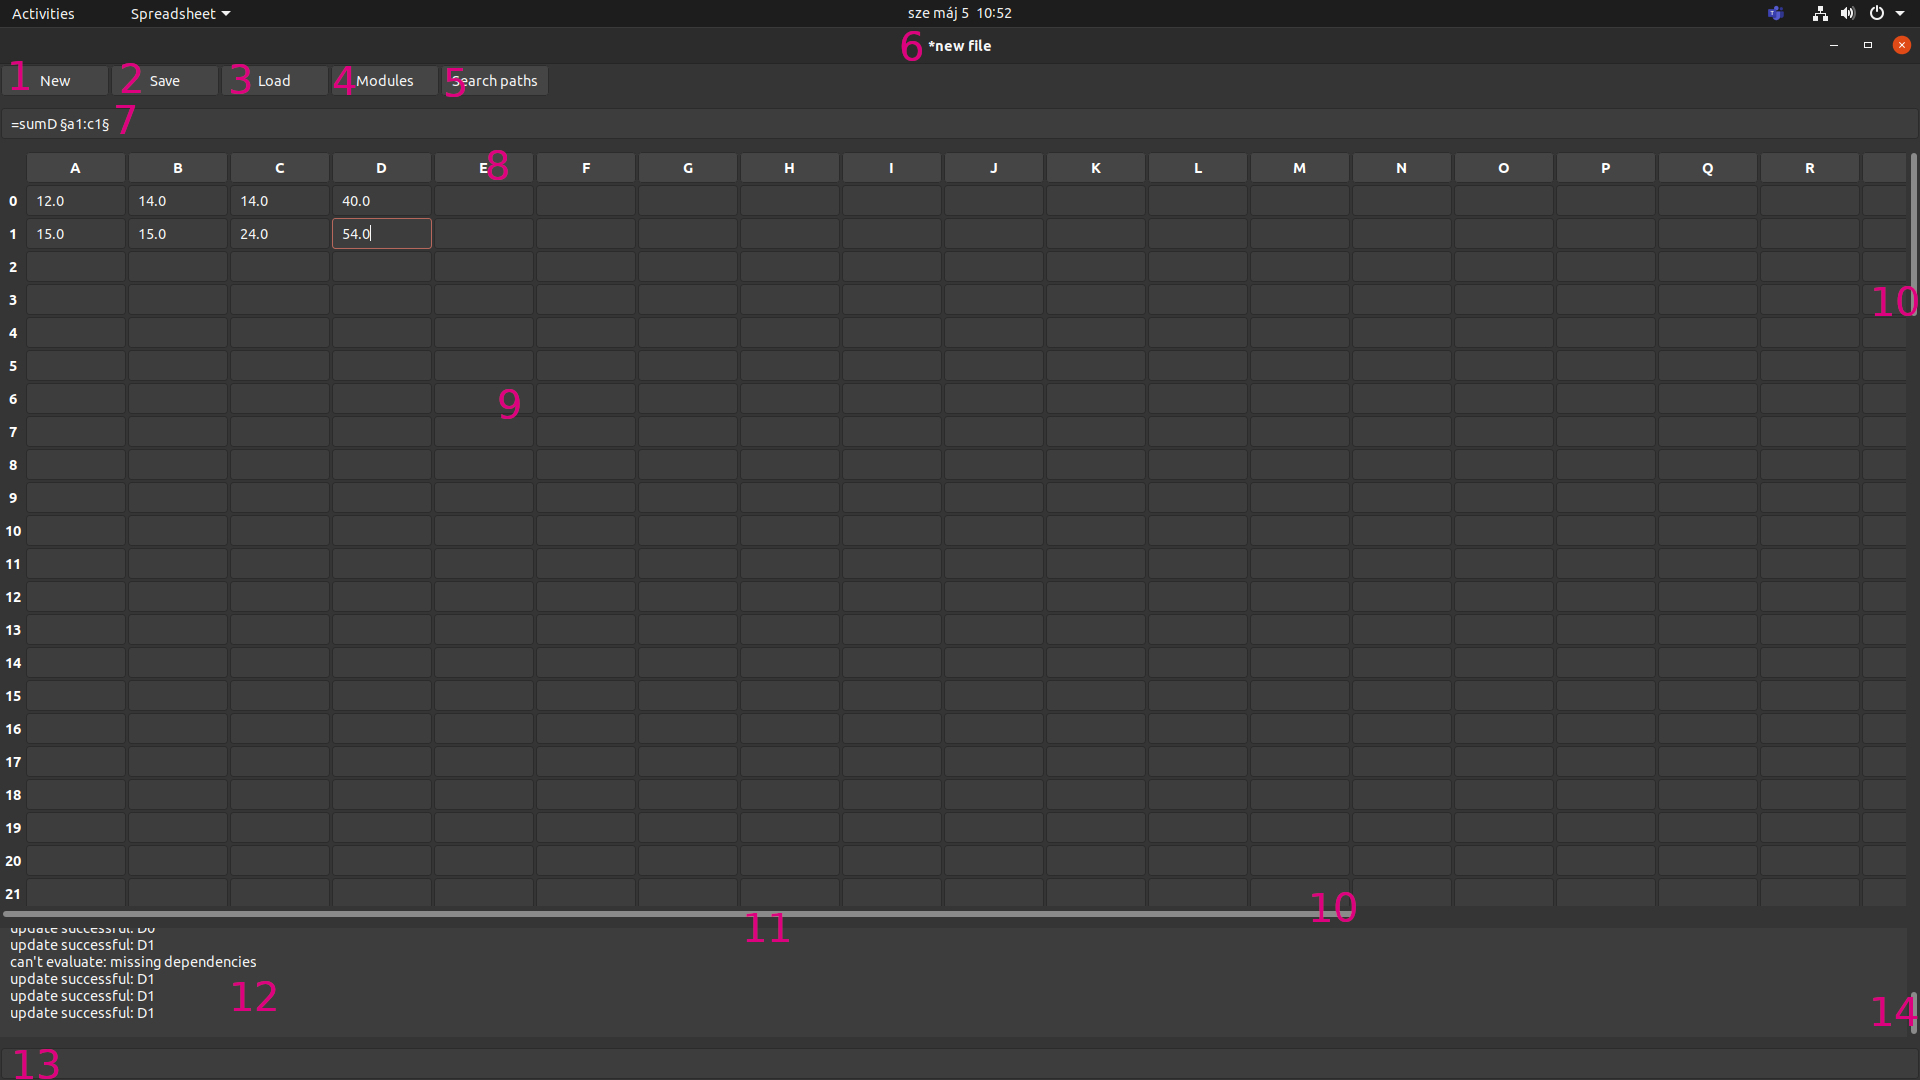
\includegraphics[width=\textwidth]{gui}
	\caption{A felhasználói felület}
	\label{fig:gui}
\end{figure}

\begin{compactenum}
	\item Ezzel a gombbal lehet új fájlt létrehozni. Ekkor a számolótábla üres lesz.
	\item Ezzel a gombbal lehet elmenteni a számolótábla aktuális állapotát. A fájl az alkalmazás saját \textit{.fsandor} kiterjesztésében kerül mentésre.
	\item Ezzel a gombbal lehet fájlt betölteni.
	\item Ezzel a menüponttal lehet beállítani a háttérben futó GHCi-be betöltendő modulok listáját. A felugró szövegmező minden sora egy modult jelent. \textbf{KELL ÁBRA?}
	\item Ezzel a menüponttal lehet beállítani, hogy az alapértelmezett útvonalakon kívül hol keresse a GHCi a betöltendő modulokat. Minden sor egy elérési útvonalat jelent. Az elérési útvonal lehet abszolút (ez utóbbi a javasolt) vagy relatív a futtatható állomány helyéhez képest.
	\item A betöltött fájl neve. Ha épp nincs elmentve a számolótábla, a "*new file" szöveg jelenik meg. Ha a betöltött fájl neve előtt szerepel egy "*", az azt jelenti, hogy a legutóbbi mentés óta történt módosítás.
	\item Kódszerkesztő. Ebbe a sorba lehet kódot írni az aktuálisan kijelölt cellához. A kijelölt cella az a cella, amelyre a felhasználó legutóbb kattintott. A beírt kód akkor kerül kiértékelésre, ha a felhasználó egy másik elemre kattint vagy leüti az entert.
	\item A számolótábla. A cellába beírt kód akkor kerül kiértékelésre, ha a felhasználó egy másik elemre kattint vagy leüti az entert.
	\item A log mutatja a végrehajtott akciók (pl. cella kódjának átírása, GHCi query eredménye) eredményét. Jobb oldalt görgethető.
	\item Az alkalmazáshoz tartozó parancssor. A beírt parancs akkor kerül kiértékelésre, ha a felhasználó leüti az entert.
\end{compactenum}

\section{Cellák és kiértékelés}

\subsection{A kifejezések}

Egy cella tartalma négyféle lehet: üres cella, szám, szöveg vagy formula. A cellába beírt kifejezés pontosan akkor formula, ha az első karaktere "=". Amennyiben az első karakter nem "=", és a beírt szöveg értelmezhető tizedestörtként, annyiban a cella tartalma számként kerül értelmezésre. Minden más esetben a cella tartalma egy string. Példák:
\begin{compactenum}
	\item Szám: "0.12", "11"
	\item Formula: "=sum [1..10]", "=§a0§+sumD §a2:b4§"
	\item String: " =sum [1..10]", "alma", ".12"
\end{compactenum}

A formulákba lehetséges cellahivatkozásokat írni. Kétféle cellahivatkozás létezik:
\begin{compactenum}
	\item Egyszerű hivatkozás. Pl: §a0§,§B1§.
	\item Listahivatkozás. Pl: §a0:B4§.
\end{compactenum}

A cellahivatkozások nem kisbetű-nagybetű érzékenyek.

A formula összes többi része Haskell kódként kerül értelmezésre. A típushelyesség a kiértékelés során kerül ellenőrzésre.

\subsection{A futásidejű reprezentáció}

Egy cella futásidejű reprezentációja egy \textit{Maybe a} típusú érték. Az üres cella reprezentációja \textit{Nothing}, a nemüres cella reprezentációja \textit{Just val}, ahol \textit{val} a cellába beírt string/szám. A kiszámított értékek is mindig Just-ba wrappelődnek, hogy y a GHCi továbbszámolhasson velük. Az értékek visszaolvasásakor ez a háttérben egy \textit{fromJust} hívással unwrappelődik.
Egész szám esetén a kódgeneráló algoritmus figyel arra, hogy olyan literált generáljon a cellaértékből, ami értelmezhető egész típusúként (azaz ilyenkor levágja a tizedesrészt).

A cellahivatkozások feloldását példákon keresztül mutatjuk be. Bal oldalt található a hivatkozás, jobb oldalt a generált kód.
\begin{compactenum}
	\item \textit{§a0§} $\rightarrow$ \textit{fromJust v0}
	\item §a0:a3§ $\rightarrow$ \textit{[v0,v2,v5,v10]}
	\item \textit{§a1:b0§} $\rightarrow$ \textit{[]}
\end{compactenum}

A cellahivatkozások feloldásakor a cellákhoz egy $\mathbb{N} \times \mathbb{N} \rightarrow \mathbb{N}$ bijekción keresztül egy azonosító kerül hozzárendelésre (innen származnak a kódban írt \textit{vi} változónevek. A függvény definíciója megtalálható a fejlesztői dokumentációban.

A fentiek alapján \textit{a} típusú cellára mutató egyszerű hivatkozás ugyanúgy használható, mint egy \textit{a} típusú érték. Az üres cellára való egyszerű hivatkozás hibát okoz. Példák (beírt kód és generált kód):
\begin{compactenum}
	\item A0 kódja: \textit{"12.0"}, B1 kódja: \textit{"=§a0§+11"} $\rightarrow$ B1 értékét kiszámító Haskell kód: \textit{v3 = Just \$ fromJust (Just 12) + 11}
	\item A0 kódja : \textit{""} B1 kódja: \textit{"=§a0§+11"} $\rightarrow$ B1 értékét kiszámító (hibát eredményező): \textit{v3 = Just \$ fromJust Nothing + 11}
\end{compactenum}

A listahivatkozások feloldásakor azonban a lista elemei \textit{Maybe a} típusúak maradnak. Példa:

A0 kódja: \textit{"12"}, A1 kódja: \textit{"13"}, A2 kódja: \textit{=sum §a0:a10} $\rightarrow$ A2 értékét kiszámító (típushibás) Haskell kód: \textit{v5 = Just \$ sum [Just 12, Just 13]}

Ez látszólag komoly problémákat eredményez, de az \textit{€} operátor (lásd 2.5.3) egy könnyen használható megoldást ad a problémára.

\subsection{Lehetséges hibák}

Egy cella kódjának megváltoztatása után előfordulhatnak hibák, az alábbiakban ezek foglaltatnak össze:
\begin{compactenum}
	\item Ha egy cella kódját nem sikerül parseolni, a cellában az "FNoParse" szöveg jelenik meg. Parseolási hiba csak formula esetén léphet fel, ha szerepel a kódban '§' karakter, de nem egy értelmes hivatkozás részeként. Példák: "=§a§", "=a1§". A Haskell szintaxis helyessége csak a kiértékelés során kerül elenőrzésre.
	\item Ha a megváltoztatott cella olyan cellára hivatkozik, amely hibás (azaz nem nyerhető ki az értéke), akkor a cellában az "FNoCache" hibaüzenet jelenik meg. 
	\item Ha a kiértékelés során hiba történt (Haskell szintaxishiba/típushiba/futásidejű hiba), akkor a cellában az és leszármazott celláiban az "FGhciError" hibaüzenet jelenik meg.
	\item Ha a cella kiértékelése egy másodpercnél tovább tart, a kiértékelés leáll, és a cellában az "FTimeoutError" szöveg jelenik meg. A leszármazott cellákban az "FGhciError" szöveg jelenik meg. Megjegyzés: a végtelen GHCi számítások terminálása nem működik teljesen megbízhatóan, így a legjobb tudatosan elkerülni az ilyen számítások futtatását. (A probléma részletes leírása megtalálható a 3.3.5 szakaszban.)
\end{compactenum}

\section{A standard könyvtár}

\subsection{Kombinátorok}

A fentiekben már láttuk, hogy \textit{a} típusú cellák listájának futásidejű reprezentációja egy \textit{[Maybe a]} típusú érték. Ez a megoldás teszi lehetővé, hogy a program kezelni tudja az üres cellákat. A probléma, ami ilyenkor felmerül, hogy egy \textit{[a] -> b} függvényt szeretnénk alkalmazni egy \textit{[Maybe a]} típusú értékre, valamilyen módon kezelve az üres cellákat.

Az első megoldás az üres cellák helyettesítése egy alapértelmezett értékkel. Erre használható az \textit{€} kombinátor:

\begin{lstlisting}[caption={Az € kombinátor}, language={Haskell},label=src:euro, escapeinside={(*}{*)}]
infix 1 (*€*)
((*€*)) :: ([a] -> b) -> a -> [Maybe a] -> b
f (*€*) b = f . map (maybe b id)
\end{lstlisting}

Példa:

\textit{"=sum € (-1) \$ §a0:a5§"} $\rightarrow$ az a0-a5 cellalista összege, üres cella esetén levon egyet az összegből.

Előfordulhat, hogy az üres cellákat egyáltalán nem szeretnénk figyelembe venni. Erre szolgál az \textit{onJusts} kombinátor:

\begin{lstlisting}[caption={Az onJusts kombinátor}, language={Haskell},label=src:gfj, escapeinside={(*}{*)}]
onJusts :: ([a] -> b) -> [Maybe a] -> b
onJusts f = f . map fromJust . filter isJust 
\end{lstlisting}

Példa:
\textit{"=onJusts (concat . map tail) §a0:a5§"} $\rightarrow$ az a0-a5 cellalista nemüres elemeinek konkatenálása, de mindegyikből elhagyva az első karaktert.

De természetesen közvetlenül is kihasználható a listahivatkozások \textit{[Maybe a]} reprezentációja. A következő kódrészlettel például megszámolhatók a nemüres cellák: \textit{"=length \$ filter isJust \$ §a0:a5§"}.

\subsection{Alapértelmezett függvénypéldányok}

Bizonyos függvényeket gyakran szeretnénk egy alapértelmezett módon használni. Például cellák összegének kiszámításához a \textit{sum € 0} függvényt, vagy cellák maximumának megkereséséhez az \textit{onJusts maximum} függvényt.

Az \textit{Empty} modul (\textbf{ÁT LESZ NEVEZVE!!}) biztosítja a \textit{Prelude} függvényeinek egy-egy az alkalmazás reprezentációjához igazított alapértelmezett változatát. Az alapértelmezett függvények neve az eredeti függvény neve és utána egy "D". Például: \textit{sumD, maximumD, foldMapD}.

\subsection{A könyvtár bővítése}

A felhasználónak lehetősége van saját modulokat írni az alkalmazáshoz, és azokat használni. (A modulok importálásáról a 2.3 szakaszban esett szó.) Saját polimorf függvények írásakor érdemes explicit kiírni a típusokat, ugyanis a monomorfizmus-megszorítás (\textbf{KELL LINK?}) miatt a Haskell fordító gyakran túl specifikus típust következtet ki. A standard könyvtár definiál két típusszinomimát listafüggvényekhez:

\begin{lstlisting}[caption={LFun és NLFun}, language={Haskell},label=src:lfun]
type LFun a b = [Maybe a] -> b
type NLFun a b = Num a => [Maybe a] -> b
\end{lstlisting}

Emellett természetesen tetszőleges Haskell modul betölthető az alkalmazásba.

\section{A parancssorban használható parancsok}

\subsection{Kifejezés kiértékelése GHCi-ban}

A program a cellák kódjának kiértékeléséhez a háttérben egy GHCi példányt futtat. Jelölje a $\_$ a szóköz karaktert és $C$ az összes karakterek halmazát. Amennyiben a beütött parancs $\_^+g\_^+C^*$ alakú, a "g"-t követő szóközök utáni részstring kiértékeltetik a GHCi-ban. A kiértékelés eredménye megjelenik log üzenetként. 

Ezen parancs segítségével lehetséges modulokat importálni és bindingokat létrehozni a GHCi által használt IO monádban. Azonban minden egyes cellakiértékelés előtt a bindingok elvesznek, a betöltött modulok pedig azok lesznek, amelyek a "Modules" menüpontban meg lettek adva. Így a gyakorlatban a GHCi ezen funkciói nem használhatók.

\subsection{Cellatartalom másolása és áthelyezése}

A \textit{cp} parancs használható cellák egy blokkjának átmásolására, az \textit{mv} parancs pedig egy cellablokk áthelyezésére. A két parancs szintaxisa nagyon hasonló formátumú: \textit{<parancs> <listahivatkozás> <egyszerű hivatkozás>}

A listahivatkozás adja meg a másolandó/áthelyezendő tartományt (bal felső és jobb alsó sarok), az egyszerű hivatkozás pedig a céltartomány bal felső sarkát. Példák:
\begin{compactenum}
	\item \textit{mv §a0:a5§ §b10§}
	\item \textit{cp §b1:c3§ §e9§}
	\item \textit{cp §a0:a3§ §a1§}
\end{compactenum}

A parancsot lehet úgy paraméterezni, hogy a kiinduló és a céltartomány átfedésben legyen (fenti 3. példa). Ebben az esetben a parancs az új értékekkel felülírja a metszetben lévő cellákat. Ha pl. a harmadik példában \textit{§a0:a4§} rendre \textit{[1,2,3,4,ÜRES]}, akkor a parancs végrehajtása után \textit{[1,1,2,3,4]} lesz a cellák tartalma.